\documentclass[UTF8]{ctexart}
\usepackage{graphicx}
\usepackage[hidelinks]{hyperref}
\usepackage{amsmath}
\usepackage{amssymb}
\usepackage{geometry}
\usepackage{booktabs}
\usepackage{enumitem}
\usepackage{float}
\usepackage{textcomp}
\usepackage{mdframed}
\usepackage[justification=centering]{caption}

\graphicspath{{../figures/}}
\geometry{a4paper, margin=1in}

\title{控制理论实用指南\\
\large 面向机器人竞赛的工程学生}
\author{Skywalker Liu\\
\href{mailto:ltx2499323877@outlook.com}{\texttt{ltx2499323877@outlook.com}} \quad\\
\quad
\href{https://github.com/liuskywalkerjskd}{\texttt{github.com/liuskywalkerjskd}}}
\date{2025年10月}

\begin{document}

\maketitle

\newpage
\tableofcontents
\newpage

%=============================================================================
\section{引言}
%=============================================================================

如果你正在读这篇文章，你大概是一个刚加入机器人竞赛战队的工科生——盯着一个死活转不到目标转速的电机，或者一个抖得像中邪了一样的云台，不知所措。欢迎。你来对地方了。

这份文档\textbf{不是}一本控制理论教材。教材固然好——严谨、全面，而且在凌晨两点能把你催眠的能力堪称一绝。这是一份\textit{学习笔记}，作者学习这些内容走的是"先把机器人搞坏，再翻理论找原因"的硬核路线。

我们的目标很简单：给你足够的理论基础，让你能够在真实硬件上\textbf{设计、调试、排查控制器}。数学该讲的还是要讲，但我们始终会问一句："当机器人上场的时候，这个到底有什么用？"

\subsection*{这份笔记写给谁看？}

低年级和中年级的本科生，尤其是参加 RoboMaster（大学生机器人对抗赛，国内最火的机器人竞赛之一）、FIRST Robotics（美国机器人大赛）、RoboCup（机器人世界杯）或类似赛事的同学。我们假设你已经学过（或正在学）微积分和基础线性代数。只要你知道导数是什么、能做矩阵乘法而不至于崩溃，你就准备好了。

\subsection*{这份笔记怎么组织的？}

我们从\textbf{数字信号处理（Digital Signal Processing）}开始——因为在你控制任何东西之前，你得先能从传感器拿到干净的数据。然后我们学如何用数学\textbf{描述系统}，说白了就是"把你的电机到底在干什么写下来"。接下来是\textbf{经典控制理论（Classical Control Theory）}，PID 就住在这里——这是竞赛机器人的看家本领。之后我们处理\textbf{离散化与工程实现（Discretization and Implementation）}，把优雅的数学和跑在固定时钟频率单片机上的残酷现实架起桥梁。最后，我们涉足\textbf{现代控制理论（Modern Control Theory）}，学习把好机器人变成优秀机器人的那些工具：LQR、MPC 和卡尔曼滤波器（Kalman Filter）。

那我们开始吧。

\newpage

%=============================================================================
\section{数字信号处理}
%=============================================================================

你可能会问："我报名学的是控制理论，怎么从信号处理开始讲？"问得好。答案是：\textbf{垃圾进，垃圾出。}

你的控制器好不好，取决于它收到的数据好不好。如果你的 IMU（惯性测量单元）读数在那里乱蹦乱跳，再怎么调 PID 参数都救不了你。所以在学会控制系统之前，我们先学怎么把信号清理干净。

\subsection{理解频域}

在日常生活中，我们用\textbf{时域（time domain）}来思考信号——电压随时间变化，位置随时间变化。这很自然，也很直觉。但事实证明，如果从另一个角度来看信号，很多问题会变得\textit{简单得多}：这个角度就是\textbf{频域（frequency domain）}。

核心思想美妙而简单：\textit{任何信号都可以分解为不同频率的正弦波之和。}你那嘈杂的陀螺仪读数？其实是一个干净的低频旋转信号，加上一堆高频噪声信号叠加在一起。如果我们能分辨出哪些频率是"有用信号"、哪些是"噪声"，就可以精准地把噪声切掉。

把它想象成音乐播放器上的均衡器（Equalizer）。低音、中音、高音都混在时域波形里。但均衡器让你可以独立地增强或衰减特定频率范围。这正是我们在控制系统中用滤波器做的事。

\textbf{关键直觉：}系统中慢速的、有意义的变化（比如底盘转向）发生在低频。快速的、没有意义的变化（比如电气噪声或振动）发生在高频。频域让我们能够把它们区分开来。

\subsection{拉普拉斯变换与傅里叶变换}

这两种变换是你从时域进入频域的通行证。它们密切相关，但用途略有不同。

\subsubsection{拉普拉斯变换}

拉普拉斯变换（Laplace Transform）将时域函数 $f(t)$ 转换为复变量 $s$ 的函数：

\begin{equation}
F(s) = \mathcal{L}\{f(t)\} = \int_0^{\infty} f(t) e^{-st} \, dt
\end{equation}

其中 $s = \sigma + j\omega$ 是复数。实部 $\sigma$ 描述指数增长或衰减，虚部 $j\omega$ 描述振荡。

\textbf{我们为什么关心它？}因为拉普拉斯变换能把微分方程变成代数方程。与其解
\[
m\ddot{x} + b\dot{x} + kx = F(t),
\]
（需要微积分），不如解
\[
(ms^2 + bs + k)X(s) = F(s),
\]
（纯代数）。导数变成乘以 $s$，积分变成除以 $s$。生活立刻轻松多了。

你每天都会用到的最重要的拉普拉斯变换对：

\begin{center}
\begin{tabular}{lll}
\toprule
\textbf{时域} & \textbf{$s$ 域} & \textbf{出现场合} \\
\midrule
$1$（阶跃输入） & $\frac{1}{s}$ & 指令一个新设定值 \\
$e^{-at}$ & $\frac{1}{s+a}$ & 一阶系统响应 \\
$\sin(\omega t)$ & $\frac{\omega}{s^2 + \omega^2}$ & 振荡、振动 \\
$\dot{f}(t)$ & $sF(s) - f(0)$ & 控制器中的微分 \\
$\int f(t)\,dt$ & $\frac{F(s)}{s}$ & 控制器中的积分 \\
\bottomrule
\end{tabular}
\end{center}

\textbf{实用建议：}你不需要背住积分公式。你需要理解的是：$s$ 意味着"求导"，$1/s$ 意味着"积分"。就这一个认知，能带你走过 80\% 的控制理论。

\textbf{$e^{-st}$ 到底在做什么？}核函数 $e^{-st} = e^{-\sigma t} e^{-j\omega t}$ 是一个"探针信号"，同时问两个问题：(1) $e^{-\sigma t}$："信号是否以速率 $\sigma$ 增长或衰减？" (2) $e^{-j\omega t}$："频率 $\omega$ 的成分有多少？"通过对 $f(t) \cdot e^{-st}$ 在全时间上积分，我们计算了信号与所有可能的指数正弦波之间的"相关性"。结果 $F(s)$ 是整个复平面的一张图，精确告诉我们信号中每种指数振荡模态各有多少。

\textbf{常用拉普拉斯变换对——推导过程：}

\textbf{单位阶跃}（Unit Step） $u(t) = 1$，$t \geq 0$：
\[
\mathcal{L}\{1\} = \int_0^{\infty} e^{-st} \, dt = \left[-\frac{e^{-st}}{s}\right]_0^{\infty} = \frac{1}{s}
\]

\textbf{指数衰减}（Exponential Decay） $e^{-at}$：
\[
\mathcal{L}\{e^{-at}\} = \int_0^{\infty} e^{-at} e^{-st} \, dt = \int_0^{\infty} e^{-(s+a)t} \, dt = \frac{1}{s+a}
\]
这就是为什么极点在 $s = -a$ 的一阶系统，其时域响应是 $e^{-at}$——极点位置\textit{就是}衰减速率。

\textbf{斜坡}（Ramp） $t \cdot u(t)$：
\[
\mathcal{L}\{t\} = \frac{1}{s^2}
\]
注意：时域乘以 $t$ 对应于对 $s$ 求导后取反号：$\mathcal{L}\{t \cdot f(t)\} = -\frac{d}{ds}F(s)$。由于 $\mathcal{L}\{1\} = 1/s$，所以 $\mathcal{L}\{t\} = -\frac{d}{ds}\frac{1}{s} = \frac{1}{s^2}$。

\subsubsection{傅里叶变换}

傅里叶变换（Fourier Transform）是拉普拉斯变换那个比较"乖"的表亲。它就是令 $s = j\omega$（即 $\sigma = 0$）时得到的结果：

\begin{equation}
F(j\omega) = \int_{-\infty}^{\infty} f(t) e^{-j\omega t} \, dt
\end{equation}

拉普拉斯变换作用于整个复平面（可以处理不稳定的增长信号），而傅里叶变换严格活在虚轴上。它告诉你："这个信号里每个频率各有多少？"

\textbf{什么时候用哪个：}
\begin{itemize}
    \item \textbf{拉普拉斯变换}：用于分析和设计控制系统（传递函数、稳定性）。
    \item \textbf{傅里叶变换}：用于分析信号（噪声、振动、频率成分）。
\end{itemize}

在实际应用中，对于数字系统，我们通常使用\textbf{离散傅里叶变换（Discrete Fourier Transform，DFT）}，并通过\textbf{快速傅里叶变换（Fast Fourier Transform，FFT）}算法高效计算。想看看传感器数据里藏着什么频率？直接扔进 FFT 就好。MATLAB 的 \texttt{fft()} 或 Python 的 \texttt{numpy.fft.fft()} 一行搞定。

\subsubsection{频谱}

对信号应用傅里叶变换后，得到的是它的\textbf{频谱（Frequency Spectrum）}——一张显示每个频率分量的幅度（和相位）的图。

读频谱就像给信号做 X 光检查：
\begin{itemize}
    \item 50 Hz 处有个高峰？那大概是工频干扰（电网噪声）。
    \item 10 Hz 以下有个宽包？那可能是你真正感兴趣的信号。
    \item 所有频率上都有随机的模糊？那是白噪声（White Noise）。
\end{itemize}

\textbf{实际案例：}假设你的云台编码器给出一个嘈杂的速度读数。你记录了 1 秒数据，计算 FFT，看到 3 Hz 处有个清晰的峰（云台正在以 3 Hz 跟踪目标），加上 50 Hz 以上一片噪声乱麻。现在你心里有数了：设计一个截止频率在 20--30 Hz 的低通滤波器，信号就会变干净。

频谱包含两部分：
\begin{itemize}
    \item \textbf{幅度谱}（Magnitude Spectrum） $|F(j\omega)|$：每个频率分量的强度。
    \item \textbf{相位谱}（Phase Spectrum） $\angle F(j\omega)$：每个频率分量的时间偏移。
\end{itemize}

在滤波器设计中，我们主要关心幅度谱。相位在后面分析控制回路稳定性（相位裕度）时才变得重要。

\begin{figure}[H]
\centering
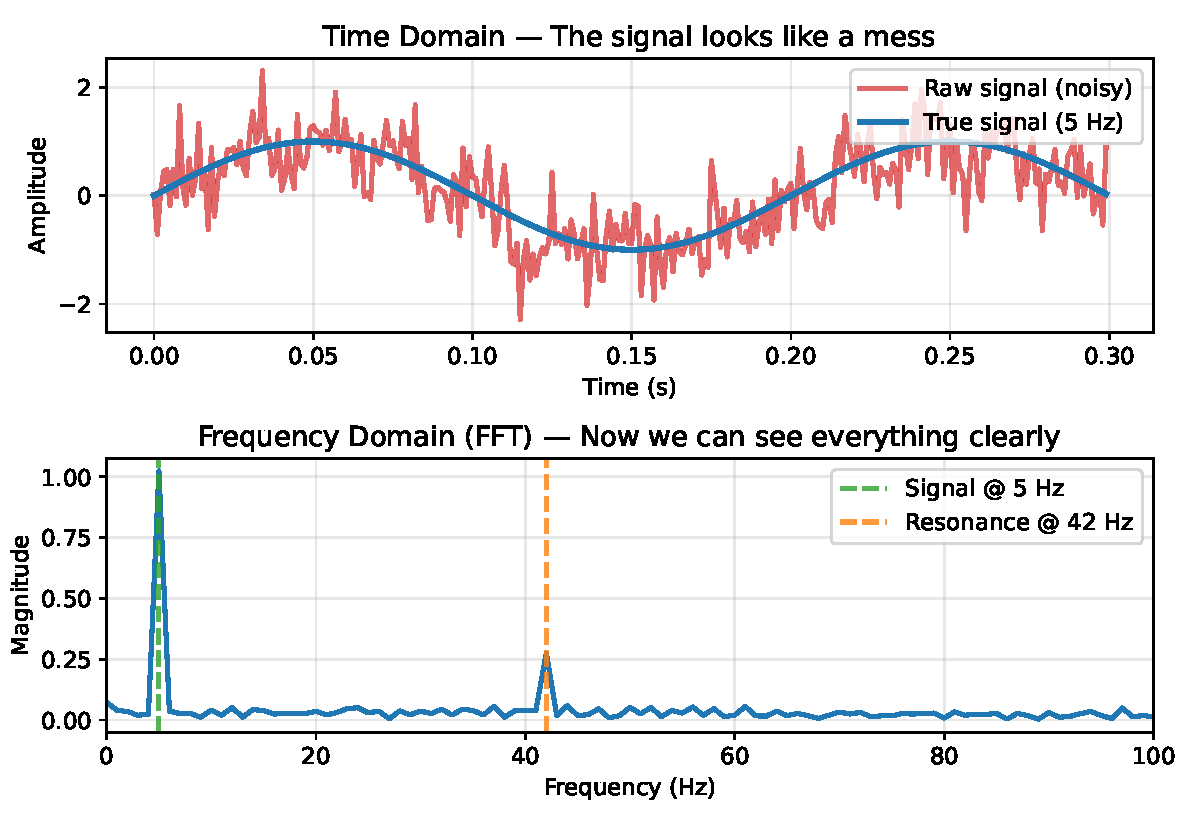
\includegraphics[width=\textwidth]{frequency_spectrum.pdf}
\caption{上图：时域中的噪声信号看起来毫无希望。下图：FFT 立刻揭示出隐藏在噪声中的 5 Hz 信号和 42 Hz 谐振。}
\end{figure}

\vspace{0.5em}
\begin{mdframed}[linewidth=1pt, innertopmargin=10pt, innerbottommargin=10pt]
\textbf{案例分析：用 FFT 排查底盘振动}

\vspace{0.3em}
这是竞赛机器人中的一个经典故障模式：你的麦克纳姆轮底盘低速跑得好好的，但高速时出现了令人抓狂的振动，整个车架嗡嗡作响。大家怀疑是螺丝松了。你把所有螺丝都拧紧了。还是振。

\textbf{诊断方法：}在出问题的速度下行驶时，记录 5 秒 IMU 加速度计数据。用 Python 跑一遍 FFT：

\begin{verbatim}
    import numpy as np
    freqs = np.fft.rfftfreq(len(data), d=1.0/sample_rate)
    spectrum = np.abs(np.fft.rfft(data))
    plt.plot(freqs, spectrum)
\end{verbatim}

你看到 42 Hz 处有个巨大的尖峰。有意思。你算了一下：高速行驶时，麦轮辊子接触地面的频率是……大约 42 Hz。辊子接触频率恰好与车架结构谐振频率吻合。

\textbf{解决方案：}
\begin{itemize}[nosep]
    \item 在控制回路中加一个 42 Hz 的\textbf{陷波滤波器（Notch Filter，带阻滤波器）}，防止控制器激励谐振。
    \item 加物理阻尼（橡胶减振垫），把谐振频率移开。
    \item 加固车架，把谐振频率推到工作频率范围以上。
\end{itemize}

\textbf{教训：}不用 FFT 的话，你可能会花好几个小时拧螺丝。用了 FFT，10 秒内根本原因一目了然。\textbf{频域是一种调试神器。}只要有什么东西在振荡而你不知道为什么，记录数据，看频谱。
\end{mdframed}

\subsection{基于频域的滤波器设计}

既然我们能在频域中"看见"信号，就可以设计滤波器——保留我们想要的频率，剔除不想要的。

滤波器本质上是一个在不同频率下增益不同的系统。我们用滤波器的\textbf{频率响应（Frequency Response）}来描述它——一张增益对频率的图（称为\textbf{波特幅度图，Bode Magnitude Plot}）。

\subsubsection{低通滤波器}

机器人中最常用的滤波器。通过低频，衰减高频。

\textbf{一阶低通滤波器（Low-Pass Filter，LPF）：}
\begin{equation}
H(s) = \frac{\omega_c}{s + \omega_c}
\end{equation}

其中 $\omega_c = 2\pi f_c$ 是截止角频率（rad/s）。低于 $\omega_c$ 的频率增益约为 1（信号通过）；高于 $\omega_c$ 的频率以 $-20$ dB/十倍频的斜率衰减（信号被压制）。

\textbf{在时域中}，这等价于一个指数移动平均：
\begin{equation}
y[n] = \alpha \cdot x[n] + (1 - \alpha) \cdot y[n-1]
\end{equation}

其中 $\alpha = \frac{T_s}{T_s + \frac{1}{2\pi f_c}}$，$T_s$ 是采样周期。

\textbf{适用场景：}平滑带噪声的传感器读数（陀螺仪、加速度计、电机电流）。这是你 90\% 的情况下会用到的滤波器。

\textbf{注意：}低通滤波器会引入\textbf{相位滞后（Phase Lag）}——输出相对于输入有延迟。滤波越激进（截止频率越低），引入的滞后越大。在快速控制回路中，这种滞后可能使系统失稳。平滑信号和快速响应之间永远存在权衡。

\begin{figure}[H]
\centering
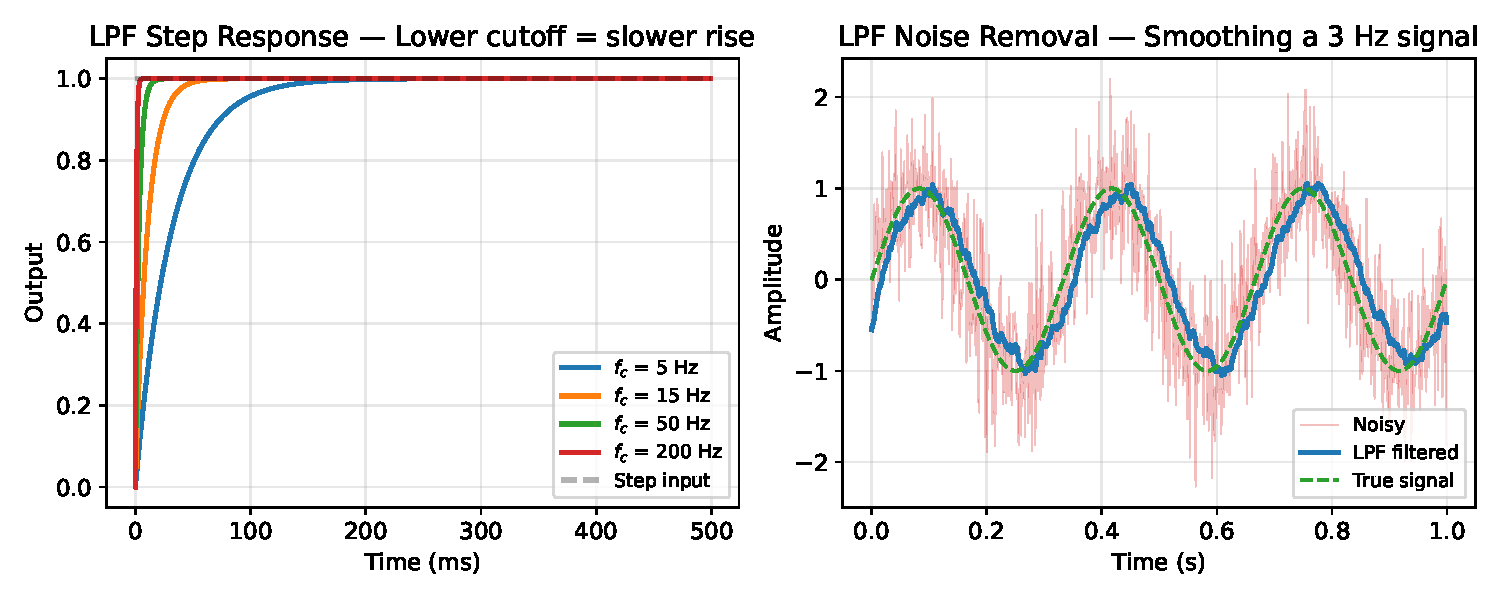
\includegraphics[width=\textwidth]{lpf_response.pdf}
\caption{左图：LPF 阶跃响应——截止频率越低，上升越慢，但输出越平滑。右图：对含噪声的 3 Hz 信号滤波——LPF 恢复出真实信号，同时去除了高频噪声。}
\end{figure}

\vspace{0.5em}
\begin{mdframed}[linewidth=1pt, innertopmargin=10pt, innerbottommargin=10pt]
\textbf{案例分析：为什么低通滤波器能免费送你"软启动"}

\vspace{0.3em}
假设你命令电机从 0 瞬间跳到 5000 RPM（阶跃输入）。没有任何滤波器的话，设定值突变——电机驱动器看到一个突如其来的全电压指令，齿轮猛地咬合，底盘猛地一窜，你的队友把咖啡洒了一地。

现在在设定值上串一个一阶低通滤波器：$r_{\text{filtered}}(s) = \frac{\omega_c}{s + \omega_c} \cdot R(s)$。会发生什么？

$s$ 域中的阶跃输入是 $R(s) = \frac{5000}{s}$。经过滤波器后：
\[
R_{\text{filtered}}(s) = \frac{5000 \, \omega_c}{s(s + \omega_c)}
\]

做拉普拉斯逆变换：
\[
r_{\text{filtered}}(t) = 5000 \left(1 - e^{-\omega_c t}\right)
\]

阶跃变成了一个\textbf{平滑的指数斜坡}。时间常数是 $\tau = 1/\omega_c$。经过 $3\tau$，输出达到目标的 95\%；经过 $5\tau$，达到 99\%。

\textbf{这对你的机器人意味着什么：}
\begin{itemize}[nosep]
    \item \textbf{机械保护：}齿轮和皮带有扭矩上限。阶跃指令可能崩掉齿轮或断掉皮带。LPF 限制了变化速率，让力保持在安全范围内。
    \item \textbf{限制涌入电流：}突然施加电压会引起巨大的涌入电流（反电动势为零时 $I = V/R$）。LPF 让电压缓慢爬升，电流保持在可控范围。
    \item \textbf{可调节的激进程度：}想要更快的斜坡？增大 $\omega_c$（提高截止频率）。想要更柔和的斜坡？减小 $\omega_c$。一个参数控制全部行为。
\end{itemize}

\textbf{与线性斜坡的对比：}你也可以让设定值线性爬升（比如每秒增加 1000 RPM）。但 LPF 更好，因为它能平滑\textit{任何}设定值的突变——不只是初始阶跃，运行过程中的突然变化也一样。这是一个"设好就不用管"的方案。

\textbf{代码极其简单：}
\begin{verbatim}
    setpoint_filtered += alpha * (setpoint_raw - setpoint_filtered);
\end{verbatim}

一行代码。没有查找表，没有状态机。这就是 LPF 作为软启动机制的魅力所在。
\end{mdframed}

\begin{figure}[H]
\centering
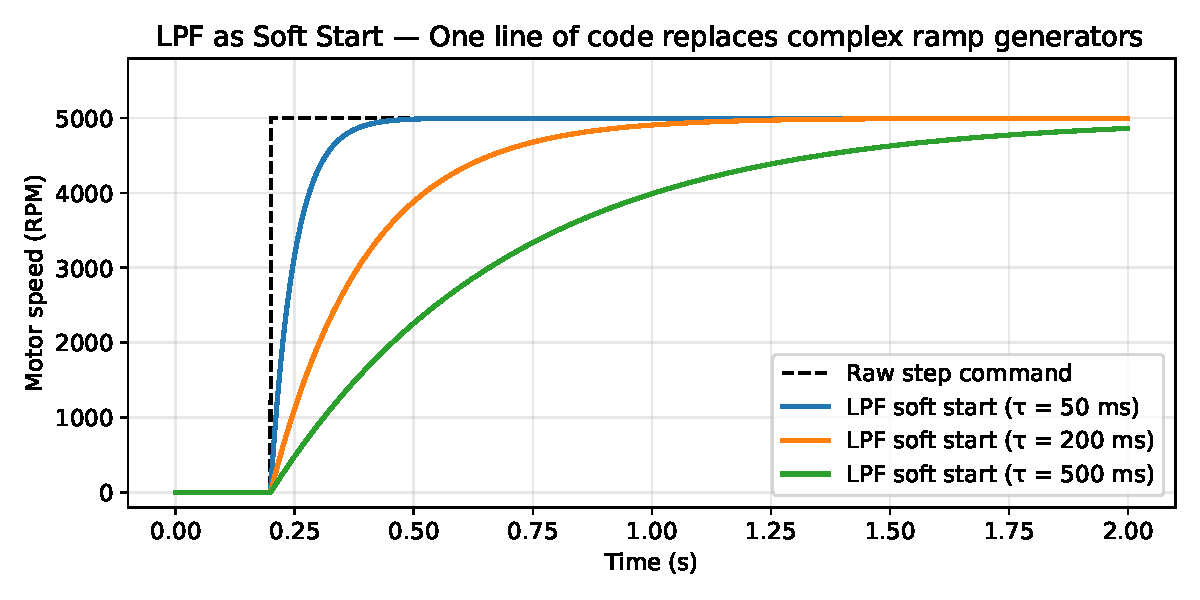
\includegraphics[width=\textwidth]{lpf_soft_start.pdf}
\caption{LPF 软启动：单个参数 $\tau$ 控制电机加速的激进程度。阶跃指令变成了平滑的指数曲线。}
\end{figure}

\subsubsection{带通滤波器}

带通滤波器（Band-Pass Filter）通过特定频率范围，衰减其他所有频率。可以看作低通和高通滤波器的组合。

\begin{equation}
H(s) = \frac{\frac{\omega_0}{Q} s}{s^2 + \frac{\omega_0}{Q} s + \omega_0^2}
\end{equation}

其中 $\omega_0$ 是中心频率，$Q$ 是品质因数（$Q$ 越高，通带越窄）。

\textbf{适用场景：}从信号中提取特定频率分量。例如，如果你知道目标在某个特定频率下振荡，想跟踪它同时剔除其他一切。

在机器人中，带通滤波器没有低通滤波器常见，但在振动分析和谐振检测方面很有用。

\subsubsection{高通滤波器}

高通滤波器（High-Pass Filter）通过高频，衰减低频。它是低通滤波器的反面。

\textbf{一阶高通滤波器：}
\begin{equation}
H(s) = \frac{s}{s + \omega_c}
\end{equation}

\textbf{适用场景：}去除信号中的直流偏置或缓慢漂移。例如，如果你的加速度计有缓慢漂移的偏置，高通滤波器可以去除它，同时保留快速加速度数据。

\textbf{实用提示：}互补滤波器（Complementary Filter，IMU 传感器融合中常用）其实就是对一个传感器做低通、对另一个传感器做高通，两者截止频率匹配使增益之和为 1。加速度计低通处理（信任它的慢速/静态姿态信息），陀螺仪高通处理（信任它的快速旋转数据）。简单、优雅，效果出奇地好。

\subsubsection{滤波器类型选择与参数整定}

选对滤波器，归根结底是回答三个问题：
\begin{enumerate}
    \item \textbf{我想保留哪些频率？}——决定滤波器类型（低通、高通、带通）。
    \item \textbf{边界在哪里？}——决定截止频率 $f_c$。
    \item \textbf{过渡要多陡？}——决定滤波器阶数。
\end{enumerate}

\textbf{经验法则：}
\begin{itemize}
    \item 从一阶低通滤波器开始。简单、稳定，大多数场合够用。
    \item 截止频率设为你感兴趣信号带宽的 5--10 倍。太低会损失信号，太高会保留噪声。
    \item 如果一阶不够，试试二阶（通带平坦用巴特沃斯（Butterworth），滚降更陡用切比雪夫（Chebyshev））。
    \item \textbf{绝对不要}在没看过实际数据频谱的情况下拍脑袋设截止频率。靠猜截止频率是挫败感的源泉。
    \item 拿不定主意时，把滤波后的输出和原始信号画在一起，检查结果是否符合物理直觉。
\end{itemize}

\subsection{Z 变换}

我们之前用拉普拉斯变换讨论的一切，都活在连续世界里。但你的单片机是数字的——它处理的是离散采样，而不是连续信号。\textbf{Z 变换（Z-Transform）}是拉普拉斯变换在离散时间中的对应物。

离散序列 $x[n]$ 的 Z 变换是：
\begin{equation}
X(z) = \sum_{n=0}^{\infty} x[n] z^{-n}
\end{equation}

关键对应关系：
\begin{center}
\begin{tabular}{ll}
\toprule
\textbf{连续域（$s$ 域）} & \textbf{离散域（$z$ 域）} \\
\midrule
$s$（导数） & $\frac{z-1}{T_s}$（前向差分） \\
$\frac{1}{s}$（积分） & $\frac{T_s}{z-1}$（累加器） \\
稳定条件 $\text{Re}(s) < 0$ & 稳定条件 $|z| < 1$ \\
$e^{-aT_s}$ 在 $s$ 域 & $z^{-1}$ 表示一个采样延迟 \\
\bottomrule
\end{tabular}
\end{center}

\textbf{我们为什么关心它？}因为当你在单片机上实现滤波器或控制器时，你实际上就是在 $z$ 域工作，不管你意识到没有。那行简单的代码：
\[
\texttt{y = alpha * x + (1 - alpha) * y\_prev;}
\]
实际上是一个 $z$ 域传递函数：
\[
H(z) = \frac{\alpha}{1 - (1-\alpha)z^{-1}}
\]

理解 Z 变换能帮你：
\begin{itemize}
    \item 把连续时间滤波器/控制器转换成代码（见第 5 节）。
    \item 分析你的离散时间系统的稳定性。
    \item 理解为什么你的控制器在不同采样频率下表现不同。
\end{itemize}

现在，只要记住一件事：\textbf{$z^{-1}$ 表示"上一个时刻"。}这是 Z 变换中最重要的一个认知。

\textbf{常用 Z 变换对：}

\begin{center}
\begin{tabular}{lll}
\toprule
\textbf{离散信号} & \textbf{$z$ 域} & \textbf{出现场合} \\
\midrule
$\delta[n]$（单位冲激） & $1$ & 初始冲击 \\
$u[n]$（单位阶跃） & $\frac{z}{z-1}$ & 阶跃指令 \\
$a^n u[n]$（等比衰减） & $\frac{z}{z-a}$ & 离散一阶系统响应 \\
$x[n-1]$（一步延迟） & $z^{-1}X(z)$ & 代码中的上一个采样值 \\
$x[n] - x[n-1]$（一阶差分） & $(1 - z^{-1})X(z)$ & 离散导数 \\
$\sum_{k=0}^{n} x[k]$（累加和） & $\frac{1}{1 - z^{-1}}X(z)$ & 离散积分 \\
\bottomrule
\end{tabular}
\end{center}

\textbf{$s$ 与 $z$ 之间的联系：}精确的映射关系是 $z = e^{sT_s}$。连续极点 $s = -a$ 映射到离散极点 $z = e^{-aT_s}$。这意味着：
\begin{itemize}
    \item 稳定的连续极点（$\text{Re}(s) < 0$）映射到 $|z| < 1$（单位圆内）。稳定性得以保持。
    \item 更快的连续极点（$s$ 更负）映射到更小的 $|z|$（更靠近原点）。极快的极点映射到 $z \approx 0$ 附近。
    \item 振荡的连续极点（$s = \sigma \pm j\omega$）映射到 $z = e^{\sigma T_s} e^{\pm j\omega T_s}$，在单位圆内（稳定）或单位圆外（不稳定）盘旋。
\end{itemize}

\textbf{读懂 $z$ 域传递函数：}任何 $z$ 域传递函数都可以直接转换成代码，只要把 $z^{-1}$ 替换成"上一个值"。例如：
\[
H(z) = \frac{b_0 + b_1 z^{-1}}{1 + a_1 z^{-1}}
\]
对应代码：
\begin{verbatim}
    y = b0 * x + b1 * x_prev - a1 * y_prev;
    x_prev = x;  y_prev = y;
\end{verbatim}
这被称为\textbf{差分方程（Difference Equation）}，是任何数字滤波器或控制器的最终形式。

\newpage

\end{document}
